\documentclass{article}
\usepackage[utf8]{inputenc}
\usepackage{referencing}
\usepackage{url, amsmath, amsthm, amssymb}
\usepackage{amsmath}
\usepackage{graphicx}
\usepackage{setspace}
\usepackage{enumitem}

\usepackage{academicons}
\usepackage{hyperref}
\usepackage{fancyhdr}
\usepackage{authblk}
\linespread{1}
\onehalfspacing
\addtolength{\oddsidemargin}{-.875in}
\addtolength{\evensidemargin}{-.875in}
\addtolength{\textwidth}{1.75in}
\addtolength{\topmargin}{-.875in}
\addtolength{\textheight}{1.75in}
\usepackage{tikz}
\usepackage[whole]{bxcjkjatype}
\usepackage{newunicodechar}
\usetikzlibrary{shapes.geometric}
\tikzstyle{V} = [circle, draw, thin, fill=white]
\tikzstyle{E} = [->, very thick]
\usepackage{amsmath,stackengine}
\stackMath
\usepackage{xfakebold}

\newcommand{\fbseries}{\unskip\setBold\aftergroup\unsetBold\aftergroup\ignorespaces}
\makeatletter
\newcommand{\setBoldness}[1]{\def\fake@bold{#1}}
\makeatother
\setBoldness{3}%

\usepackage{multicol}
\usepackage{hyperref}
\usepackage{mathrsfs}
\usepackage{abstract}
\hypersetup{
    colorlinks,
    citecolor=black,
    filecolor=black,
    linkcolor=black,
    urlcolor=black
}
\newcommand{\makeset}[2]{\left\lbrace #1 \;\middle|\;
  \begin{tabular}{@{}l@{}}
    #2
   \end{tabular}
  \right\rbrace}


\newcommand{\N}{\mathbb{N}}
\newcommand{\End}{\operatorname{End}}
\newcommand{\mb}[1]{\mathbb{#1}}
\newcommand{\mc}[1]{\mathcal{#1}}
\newcommand{\bl}[1]{\mathbf{#1}}
\newcommand{\nthpow}[1]{#1^\mb{N}}
\newcommand{\cont}{\mathfrak{c}}
\newcommand{\es}{\varnothing}
\newcommand{\amal}[3]{#1\cup_{#3}#2}
\renewcommand{\a}{\alpha}
\renewcommand{\l}{\lambda}
\newcommand{\im}{\operatorname{img}}
\newcommand{\tree}{\operatorname{tree}}
\newcommand{\leaves}{\operatorname{leaves}}
\newcommand{\cone}{\operatorname{cone}}
\newcommand{\dom}{\operatorname{dom}}
\DeclareMathOperator{\pst}{pst}
\DeclareMathOperator{\PEnd}{PEnd}
\DeclareMathOperator{\tot}{tot}
\DeclareMathOperator{\rt}{root}
\DeclareMathOperator{\shrub}{shrub}

\title{Finite Presentability of Brin-Higman-Thompson Monoids via Free J\'{o}nsson-Tarski Algebras}
\author{Bill de Witt, Luke Elliott}

\begin{document}
\maketitle


%Add in reference from collin (before def 3.4)

%(intermediate text).


%NOTE FOR US: our prefix code=birget maximal joinless code (mention this)

%Acknowledge

% shooting for march


%Lawson paper reference \cite{lawson2021polycyclic}?



% Arxiv.

% publish.

% think about alternative for n-dimensional JK algebras

% Think about partial (and all submonoids).

\begin{abstract}
    We show that the  total monoids \(totnM_{k,1}\) introduced by Birget \cite{birget2020monoid, birget2009monoid}(and their multi-rooted generalisations), which extend the Brin-Higman-Thompson groups, can be realised as the endomorphism monoids of higher dimensional J\'onnson-Tarski algebras. 
    We use this representation to show that they are finitely presented.
\end{abstract}
\tableofcontents
\section{Introduction}

A monoid version of \(V\) was first considered by Thompson (Thompson has given talks about this monoid, but to our knowledge he has not published about this).

Birget describes in \cite{birget2009monoid} several monoid extensions \(M_{k,1}\) of the well studied groups \(G_{k,1}\). These involve, in simplified terms, replacing the bijective `prefix exchange' maps of \(G_{k,1}\) with partial maps on prefix codes which need not be injective or have incomparable image sets. He also introduced the submonoids: \(sur M_{k,1}\) using partial functions whose range contains a complete prefix code; \(tot M_{k,1}\) using non-partial functions; and \(Inv M_{k,1}\) using partial functions with incomparable image set. The monoid considered by Thompson was \(totM_{2,1}\).

Birget then in \cite{birget2020monoid} extended the definition to higher dimensional analogs \(nM_{k,1}\) which extend \(nG_{k,1}\), and it is easy to see that the aforementioned submonoids extend in the same manner. We deal with the multi-rooted generalisations \(tot nM_{k,r}\) of the non-partial monoids.

The variety of J\'onsson-Tarski algebras were first introduced in \cite{jonsson1961two} as an example of a variety whose free objects have some unusual properties (related to generation of the free objects). Some work has been done on generalisations of the concept, such as in \cite{dudek1979universal,goetz1960bases} which defines varieties \(\mc{A}_{m,n}\). For our purposes we will use \(\mc{A}_{1,n}\) and higher dimensional analogues which are not equivalent to \(\mc{A}_{m,n}\) for dimension \(m\).

Higman worked with J\'onsson-Tarski algebras and the generalisations \(G_{n,r}\) in \cite{higman1974finitely}, and this is extended by Mart\'{i}nez-P\'{e}rez and Nucinkis in \cite{martinez2013bredon}. It is our understanding that Higman defined \(G_{n,r}\) as automorphism groups of \(r\) generated free algebras in the varieties \(\mc{A}_{1,n}\). We show that analogously,  \(totnM_{k,r}\) is the endomorphism monoid of an \(r\) generated free algebra:

%\cite{birget2009monoid}
\begin{theorem}[Main Theorem 1]
For \(r,n,k\in\mb{N}\), with \(r, n\geq 1\) and \(k\geq 2\), then the following monoids are isomorphic:
\begin{enumerate}
    \item [\textit{i)}]\(totnM_{k,r}\).
    \item [\textit{ii)}] The endomorphism monoid of an \(r\) generated free algebra in an \(n\)-dimensional \(k\)-ary J\'onsson-Tarski variety. 
\end{enumerate}
\end{theorem}
\begin{theorem}[Main Theorem 2]
For \(r,n,k\in\mb{N}\), with \(r, n\geq 1\) and \(k\geq 2\), the monoid \(totnM_{k,r}\) is finitely presented.
\end{theorem}

\begin{center}
    
{Acknowledgements}

We would like to thank Matt Brin and Collin Bleak for their input and advice in the construction of this paper. In particular the proof of the finite presentability results in this paper where based off of Thompson's original proof in the one dimensional case which we were made aware of by Matt Brin.
\end{center}

\section{Definitions of Objects}

In this section we will introduce the definitions of the relevant monoids, as well as a number of other useful objects. We will keep these definitions brief but for a more detailed definition for \(totM_{k,1}\), see \cite{birget2009monoid}. Some notes on notation, for the purposes of this paper: 
\begin{itemize}

\item \(0\in\N\),
\item \(\omega=|\N|\),
\item functions act on the right,
\item we treat tuples as functions, i.e. if \(x\) is a tuple (or word) we use \((i)x\) to refer to the \(i\)th element of \(x\) (indexed from \(0\)),
\item for a function \(f\), we denote by \(f|_{A}\) the restriction of \(f\) to \(A\),
\item for functions \(f,g\), we use the notation \(f^{g}=g^{-1}\circ f \circ g\).
\end{itemize}


\begin{definition}
Let \(nT_{k,r}:=\{0, 1, \ldots, r-1\}\times (\{0, 1, \ldots, k-1\}^*)^n\).
\end{definition}

This is the \(r\)-rooted, \(n\)-dimensional \(k\)-ary analog of the usual binary tree. Note that this is not always tree, for instance in \(2T_{2,1}\), we have \((0,(\varepsilon,\varepsilon)),(0,(\varepsilon, 0)), (0,(0,\varepsilon)),(0,(0,0))\) which form a cycle.

\begin{definition}
If \(k\geq 2\) and \(n\in\mathbb{N}\), then we define \(\mathfrak{C}_{n, k}:=(\{0, 1, \ldots, k-1\}^\omega)^n\) to be the \(k\)-ary \(n\)-dimensional cantor space.
Moreover if \(r \geq 1\), then we define \(\mathfrak{C}_{n, k, r}:=\{0, 1, \ldots, r-1\}\times \mathfrak{C}_{n, k}\) to be the \(r\)-rooted \(k\)-ary \(n\)-dimensional cantor space with the usual product topology.
\end{definition}

Note that topologically, these spaces are all homeomorphic. That's not relevant, but it's kinda neat. Actually relevant is that they are compact, and have a basis consisting of clopen sets (specifically the cones as defined \ref{def:cones}).

\begin{definition}
An element of \((\{0, 1, \ldots, k-1\}^*)\) or \(\{0, 1, \ldots, k-1\}^\omega)\) is a \textit{word}.
An element of \((\{0, 1, \ldots, k-1\}^*)^n\) or \(\{0, 1, \ldots, k-1\}^\omega)^n\) is a \textit{shrub}.
An element of \(nT_{k,r}\) or \(\mathfrak{C}_{n,k,r}\) is called a \textit{shrubbery}.
Note that a shrubbery is a pair, the first entry being the \textit{root} of the shrubbery, and the second a shrub. We denote the root and shrub of a shrubbery \(w\) by \(\rt(w)\) and \(\shrub(w)\) respectively. 
We define the \textit{depth} \(d(w)\) of a shrub \(w\) to be the least \(k\in \N \cup\{\omega\}\) such that for all \(i<n\) we have \(|(i)w| \leq k\).
We define the \textit{depth} \(d(w)\) of a shrubbery \(w\) to be the depth of the corresponding shrub \(\shrub(w)\).
We say that a shrub \(s\) is \textit{flat}, if all the words in \(s\) have length \(d(s)\).
We say that a shrubbery is \textit{flat}, if the corresponding shrub is flat.
\end{definition}

Notation: If \(u\) is a finite shrubbery and \(v\) is shrub, then we use \(uv\) to denote the shrubbery with the same root as \(u\) and such that the words in the shrub of \(uv\) are the words obtained by concatenating the words in the shrub of \(u\) with the words in \(v\) coordinate wise.

\begin{definition}
For words \(u,v\) we say \(u\leq v\) if \(u\) is a prefix of \(v\).
For shrubberies \(u,v\) we say \(u\leq v\) if \(\rt(u)=\rt(v)\) (i.e. they have the same root), and for all \(i\), \((i)\shrub(u)\leq(i)\shrub(v)\) (i.e. the \(i\)th word in \(u\) is less than the \(i\)th word in \(v\).
\end{definition}

The relation \(\leq\) is a partial order on shrubberies. In pictorial representations, when \(a\leq b\), \(b\) will be below \(a\).

\begin{definition}\label{def:cones}
Let \(w\in nT_{k, r}\). We define the cone under \(w\) as 
\[\cone(w):= w \mathfrak{C}_{n, k}=\makeset{wu}{\(u\in \mathfrak{C}_{n, k}\)}=\makeset{u\in \mathfrak{C}_{n, k, r}}{\(u\geq w\)}.\]
i.e. it is the set of shrubberies in \(\mathfrak{C}_{n,k,r}\) with the same root as \(w\), and such that each word in the shrub of the shrubbery has the corresponding word in the shrub of \(w\) as a prefix.
\end{definition}

Equivalently this is the boundary of the upwards closure of \(w\) in \(nT_{k,r}\).

\begin{definition}
For a finite subset \(S\) of \(nT_{k, r}\), we define \(\leaves(S)\) to be the set of maximal shrubberies of \(S\).
A pseudotree \(T\) of \(nT_{k,r}\) is a finite downwards closed (with respect to the shrubbery order) subset such that the cones of the leaves of \(T\) partition \(\mathfrak{C}_{n,k,r}\).
The \textit{depth} of \(T\) is \(d(T)=\max\makeset{d(w)}{\(w\in T\)}\).
\end{definition}

In other words, the depth of \(T\) is the length of the longest word in the shrubs of the shrubberies of \(T\). Again, note that a pseudotree is not necessarily a tree (unless \(n,r=1\)).

\begin{definition}
For a topological space \(A\), we define \(\End(A)\) to be the monoid of continuous functions from \(A\) to itself.
\end{definition}

This is the endomorphism monoid of \(A\), which is the monoid analog of the automorphism group.

\begin{definition}
We define a monoid \(tot nM_{k,r}\) to be the set \(f\in\End(\mathfrak{C}_{n, k,r})\), represented by pairs \((D,h)\) where \(D\) is a pseudotree of \(nT_{k,r}\), and \(h: \leaves(D)\to nT_{k,r}\).
Define \(\tilde{h}\) to be the partial function from \(nT_{k,r}\to nT_{k,r}\) which extends \(h\) such that \((dw)\tilde{h}=(d)hw\) for all \(d\in\leaves(D)\) and shrubs \(w\).
\end{definition}

This algebra is equivalent to \(tot M_{k,1}\) as defined by Birget in \(\cite{birget2009monoid}\) for \(n,r=1\). It is also equivalent to the subalgebra of \(nM_{k,1}\) defined in \(\cite{birget2020monoid}\) containing only the total functions. Comparing this to a common definition of \(nG_{k,r}\), where we map the leaves of a pseudotree via a bijection to the leaves of another psuedotree, here we can map the leaves of of a psuedotree to any set of shrubberies.

In \cite{jonsson1961two}, they define a variety \(K_2\), which was constructed specifically to not have the properties: 
\begin{enumerate}
    \item An algebra in a variety \(K\) which is freely generated by a finite set, cannot be generated by a set with fewer elements;
    \item If algebra in a variety \(K\) is freely generated by a finite set, then any generating set of the same size is a free generating set.
\end{enumerate}

We now define the \(n\)-dimensional \(k\)-ary J\'{o}nnson-Tarski varieties (\(nJ_k\)) that we will use for our main theorem. These varieties have appeared before in \cite{martinez2013bredon}. 
The idea of a 1-dimensional J\'{o}nnson-Tarski variety is to represent bijections from \(A^k\) to \(A\)  for some set \(A\), so we have a \(k\)-ary operation (the bijection) and \(k\) unary operation which 'undo' the \(k\)-ary operation. It is not difficult to see that the general \(nJ_k\) also do not have properties 1. and 2. and this will come up in later proofs.

\begin{definition} \label{def:nVk}
Let \(n\mc{J}_{k}\) be the variety of algebras with \(n\) \(k\)-ary operations \((\l_i)_{i<n}\) and \(nk\) unary operations \((\a_{i,j})_{i<n, j<k}\), satisfying the following equations:
\begin{enumerate}
    \item[\textit{i)}] \((x\a_{i,0},\dots,x\a_{i,k-1})\l_i=x\) for all \(x\) and \(i<n\),
    \item [\textit{ii)}] \((x_0,\dots,x_{k-1})\l_i\a_{i,j}=x_i\) for all \(x_0,\dots,x_{k-1},j<k\),
    \item [\textit{iii)}] \(\alpha_{i, l}\alpha_{i', m} =\alpha_{i', m}\alpha_{i, l}\) for all \(i,i'<n\) with \(i\neq i'\) and \(l,m<k\).
\end{enumerate}
\end{definition}

We would also naturally want the identities given in the following proposition to hold in the variety \(n\mc{J}_{k}\) (and we use them later in the paper), we do not include them in the definition as they are longer and are consequences of the given identities.
\begin{proposition}\label{prop:nVk1}
Suppose that \(A\) is an algebra in the variety \(n\mc{J}_k\), for all \(a, b < k\), \(x_a,x_{a, b}\) are elements of \(A\), \(i,i'<n\), and \(l, m<k\):
\begin{enumerate}
    \item [\textit{i)}] \((x_0,\dots,x_{k-1})\l_i\a_{i', l}\a_{i,m}=x_{m}\a_{i', l}\)\\
    \item [\textit{ii)}] \((x_0\a_{i', l},\dots,x_{k-1}\a_{i', l})\l_i=(x_0,\dots,x_{k-1})\l_i\a_{i', l}.\)\\
    \item [\textit{iii)}]\(((x_{0,0},\dots,x_{0,k-1})\lambda_i,\dots,(x_{k-1,0},\dots,x_{k-1,k-1})\l_i)\l_{i'}=((x_{0,0},\dots,x_{k-1,0})\lambda_{i'},\dots,(x_{0,k-1}\dots,x_{k-1,k-1})\l_{i'})\l_i.\)
\end{enumerate}
\begin{proof}

i) By Definition \ref{def:nVk} \textit{iii)} and then \textit{ii)}:
\[(x_0,\dots,x_{k-1})\l_i\a_{i', l}\a_{i,m}=((x_0,\dots,x_{k-1})\l_i\a_{i,m})\a_{i',l}= x_{m}\a_{i', l}.\]

ii) Using i), we can substitute \(x_m\a_{i',l}\) with \((x_0,\dots,x_{k-1})\l_i\a_{i', l}\a_{i,m}\), and then we can use Definition \ref{def:nVk} i):
\begin{align*}
   (x_0\a_{i', l},\dots,x_{k-1}\a_{i', l})\l_i&=
((x_0,\dots,x_{k-1})\l_i\a_{i', l}\a_{i,0},\dots,(x_0,\dots,x_{k-1})\l_i\a_{i', l}\a_{i,k-1})\l_i\\
&=(x_0,\dots,x_{k-1})\l_i\a_{i', l}. 
\end{align*}

iii) Let \[L := (x_{0,0},\dots,x_{0,k-1})\lambda_i,\dots,(x_{k-1,0},\dots,x_{k-1,k-1})\l_i)\l_{i'},\] 
\[R:=((x_{0,0},\dots,x_{k-1,0})\lambda_{i'},\dots,(x_{0,k-1}\dots,x_{k-1,k-1})\l_{i'})\l_i.\] 
We show that \(L=R\).

Note that \(L\a_{i,l}\a_{i',m}=L\a_{i',m}\a_{i,l}=x_{m,l} = R\a_{i,l}\a_{i',m}\) via application of Definition \ref{def:nVk} iii) and ii)
for all \(l, m<k\). Thus for all \(l<k\)
\begin{align*}
    L\a_{i,l}&= (L\a_{i,l}\a_{i',0},L\a_{i,l}\a_{i',1},\ldots, L\a_{i,l}\a_{i',k-1})\l_{i'} \\
    &= (R\a_{i,l}\a_{i',0},R\a_{i,l}\a_{i',1},\ldots, R\a_{i,l}\a_{i',k-1})\l_{i'} \\
   &= R\a_{i,l}.
\end{align*}
Similarly
\begin{align*}
    L&= (L\a_{i,0},L\a_{i,1},\ldots, L\a_{i,k-1})\l_{i} \\
    &= (R\a_{i,0},R\a_{i,1},\ldots, R\a_{i,k-1})\l_{i} \\
   &= R.
\end{align*}
\end{proof}
 
\end{proposition}

\begin{figure}
    \centering
    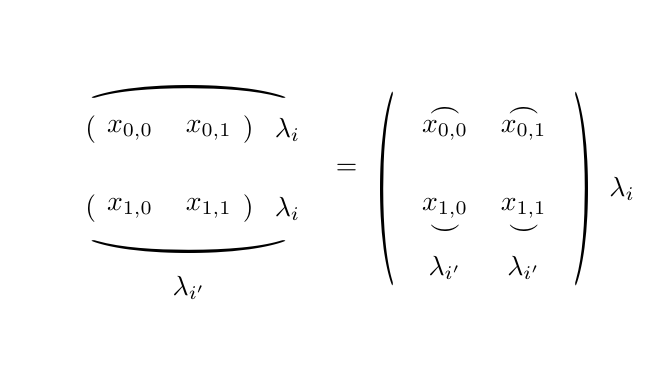
\begin{tikzpicture}
        \foreach \x/\y/\place in {{0/0/(0,0)},{0/1/(1,0)},{1/0/(0,-1)},{1/1/(1,-1)}}
            \node (l\x\y) at \place {\(x_{\x,\y}\)};
        \foreach \x/\y/\place in {{0/0/(4,0)},{0/1/(5,0)},{1/0/(4,-1)},{1/1/(5,-1)}}
            \node (r\x\y) at \place {\(x_{\x,\y}\)};
        \foreach \i/\place in {{1/(-0.5,0)},{2/(-0.5,-1)}}
            \node (lb) at \place{(};
        \foreach \i/\place in {{1/(1.5,0)},{2/(1.5,-1)}}
            \node (rb) at \place{)};
        \foreach \place in {{(2,0)},{(2,-1)},{(6.25,-0.75)}}
            \node (li) at \place{\(\lambda_i\)};
        \foreach \place in {{(4,-1.75)},{(5,-1.75)},{(0.75,-2)}}
            \node (li') at \place{\(\lambda_{i'}\)};
        \node (e) at (2.75,-0.5){=};
        \node[rotate=90,yscale=7,xscale=2] (BB1) at (0.75,0.5){)};
        \node[rotate=-90,yscale=7,xscale=2] (BB1) at (0.75,-1.5){)};
        \node[yscale=7,xscale=2] (BB1) at (5.75,-0.75){)};
        \node[rotate=180,yscale=7,xscale=2] (BB1) at (3.25,-0.75){)};
        \node[rotate=90] (BB1) at (4,0.25){)};
        \node[rotate=90] (BB1) at (5,0.25){)};
        \node[rotate=-90] (BB1) at (4,-1.25){)};
        \node[rotate=-90] (BB1) at (5,-1.25){)};
    \end{tikzpicture}
    \caption{Pictoral representation of Proposition \ref{prop:nVk1} iii)}
    \label{fig:prop:nVK1iii}
\end{figure}

The algebras we use in the main theorem are the free algebras in these varieties. The free algebra is a construction that you can do in any variety, but we define them specifically.

\begin{definition}
For each \(k\geq 2\), \(r\geq 1\) and \(n\in\mathbb{N}\), let \(\mb{F}_{n,k,r}\) be the free algebra (in the variety \(n\mc{J}_{k}\)) with free generating set \(\{0,1 ,\ldots, r-1\}\).

That is if \(nA_{k, r}\) is the algebra such that
\begin{enumerate}
    \item the strings \(0, 1, \ldots, r-1\) are elements of \(nA_{k, r}\),
    \item if \(x_0, x_1, \ldots, x_{k-1}\in nA_{k, r}\) and \(d<n\), then the string \((x_0, x_1, \ldots, x_{k-1})\lambda_d \in nA_{k, r}\), 
    \item if \(x\in nA_{k, r}\) \(d<n\) and \(j<k\), then the string \((x)\alpha_{d, j}\in nA_{k, r}\),
\end{enumerate}
(where \((, ), \alpha_{d, j}, \lambda_d,\) and comma are treated as symbols for \(d<n\) and \(j<k\))
and nothing else is an element of \(nA_{k, r}\) (with the obvious operations).
Then \(\mb{F}_{n,k,r}\) is the quotient of \(nA_{k,r}\) by the least congruence \(\sim\) containing the relations defining \(n\mc{J}_{k}\).
For brevity, from now on we will use an element of \(nA_{k,r}\) to denote the \(\sim\)-class of the element.
\end{definition}

\begin{lemma}
If \(x\in \mb{F}_{n,k, r}\) is arbitrary, then there is an element of \(nA_{k, r}\) representing it which doesn't have \(``\lambda_{d_0})\alpha_{d_1,i}"\) as a contiguous substring for any \(d_0, d_1<n\) and \(i<k\).
\end{lemma}
\begin{proof}
This is immediate from Definition \ref{def:nVk} ii) and Proposition \ref{prop:nVk1} ii).
\end{proof}

With the preceding definition and lemma, we now have a (non-unique) form by which we can represent elements of \(\mb{F}_{n,k,r}\), with `all the lambdas at the end' (note that the lambdas aren't actually at the end of the string, but that they are applied last in the path from generators to represented element).

\begin{definition}
\(\End(\mb{F}_{n,k,r})\) is the endomorphism monoid of \(\mb{F}_{n,k,r}\).
\end{definition}

This is the second of the monoids from the main theorem that we will be working with.

\section{Constructing the Isomorphism}

Now we can start work on developing the tools with which we can prove the main theorem. We start with a natural embedding of the \(nT_{k,r}\) into our free algebras: the idea is mapping roots to the free generators, and the shrubs attached to the roots correspond with applying unary operations in the algebra.

\begin{definition}
Define a map \(\tree_{n,k,r}:nT_{k,r}\to \mb{F}_{n,k,r}\) by \[(m,(s_0, s_1, \ldots, s_{n-1}))\tree_{n,k,r}=(m)\prod_{i=0}^{n-1}\prod_{j=0}^{|s_i|-1}\a_{i,(j)s_i}\]

Equivalently, let \(\phi: (\{0, 1, \ldots, k-1\}^*)^n \to \makeset{f}{\(f:\mb{F}_{n,k,r} \to \mb{F}_{n,k,r}\) }\) be the unique semigroup homomorphism such that for all \(i<n\) and \(j<k\), \(\phi\) sends the shrub with a \(j\) in the \(i\)th coordinate, and the empty word in all other coordinates to \(\alpha_{i, j}\). 
Then define the map \(\tree_{n,k,r}:nT_{k,r}\to \mb{F}_{n,k,r}\) by
\[(m,s)\tree_{n,k,r}= (m)((s)\phi).\]
We also extend the definitions of depth and flat to \(\im(\tree_{n, k, r})\) via the map \(\tree_{n, k, r}\).
\end{definition}

One very natural notion in \(nT_{k,r}\) is complete prefix codes. In the 1-dimensional case, this is equivalent to a complete antichain in the order on the words, however we need a slightly different condition for complete prefix codes to be useful. Birget refers to these as maximal joinless codes in \cite{birget2009monoid,birget2020monoid}, but we will use the term complete prefix code, as is common in works on the 1-dimensional Higman-Thompson groups.

\begin{definition}
A \textit{complete prefix code} \(A\) is a subset of \(nT_{k,r}\) such that \(\{\cone(l):l\in A\}\) is a partition of \(\mathfrak{C}_{n,k,r}\). A \textit{prefix code} is a subset of a complete prefix code.
\end{definition}

\begin{remark}
Complete prefix codes are finite (because cantor space is compact and hence any open partition of cantor space is finite).
\end{remark}

Complete prefix codes are in bijective correspond with pseudotrees. In particular, the leaves of any pseudotree are a complete prefix code, and every complete prefix code is the leaves of a pseudotree.

\begin{definition}
    If \(A\subseteq nT_{k,r}\) is a complete prefix code, then we define a pseudotree \(\pst(A)\) as the unique pseudotree whose maximal elements are \(A\).
\end{definition}

We obtain \(\pst(A)\) by taking the downwards closure (with respect to the order on shrubberies) of \(A\). It is obvious that this yields a unique pseudotree.

We can manipulate complete prefix codes via expansions. This idea is not new, and is used commonly in work with Higman-Thompson groups and their extensions, for instance in \cite[Lemma 3.3]{lawson2021polycyclic}.
More specifically, using expansions to modify free generating sets of J\'onsson-Tarski algebras in done in Chapter 2 of \cite{higman1974finitely}.

\begin{definition}
Let \(M\) be a multisubset of \(nT_{k,r}\), \(a\in M\) and \(w=(i)\shrub(a)\) for some \(i<n\).
For each \(0\leq l<k\) define \(a_l\in nT_{k,r}\) to be such that \(\rt(a_l)=\rt(a)\), \((i)\shrub(a_l)=wl\) and for all \(i'\neq i\) \((i')\shrub(a_l)=(i')\shrub(a)\). 
An elementary expansion of \(M\) about \(a\) in dimension \(i\) is a multiset which can  be obtained from \(M\) by removing one copy of \(a\) from \(M\) and adding a copy of each element of \(\{a_l:0\leq l<k\}\).
\end{definition}

\begin{definition}
An expansion \(E\) of a multiset \(M\) is a multiset which can be constructed from \(M\) via a finite sequence of elementary expansions.
We extend the definitions of (elementary) expansions to multi-subsets of \(\im(\tree_{n, k, r})\) via the map \(\tree_{n, k, r}\).
\end{definition}

\begin{lemma}\label{lem:FreeGenExpansion}
If \(M\) is a finite multisubset of \(nT_{k, r}\) and \(E\) is an elementary expansion of \(M\), then the multiset \((M)\tree_{n, k, r}\) is a free generating set for \(\mb{F}_{n,k, r}\) if and only if the multiset \((E)\tree_{n, k, r}\) is a free generating set for \(\mb{F}_{n,k, r}\). 
\end{lemma}
\begin{proof}
\((\Rightarrow)\) Suppose that \(E\) is obtained from \(M\) and \(\{a_l:0\leq l<k\}\) as an elementary expansion of \(a\) in dimension \(i\) (as in the definition of an elementary expansion). 
Let \(\Gamma\) be an algebra in the variety \(n\mc{J}_{k}\) and let \(\phi: (E)\tree_{n, k, r} \to \Gamma\) be a function.
It suffices to show that \(\phi\) extends uniquely to a homomorphism.
Let \(\phi':(A)\tree_{n, k, r} \to \Gamma\) be the function with agrees with \(\phi\) where possible and such that 
\[(a)\phi' = ((a_0)\phi, \ldots, (a_{k-1})\phi)\lambda_i.\]
By the universal property, the map \(\phi'\) extends to a unique homomorphism \(\tilde{\phi}: \mb{F}_{n,k, r}\to \Gamma\). By definition of \(\phi'\), it follows that \(\phi \subset \tilde{\phi}\).
Hence \(\phi\) extends to a homomorphism, note that all extensions of \(\phi\) to a homomorphism are also extensions of \(\phi'\) and hence this homomorphism is unique.

\((\Leftarrow)\) This follows by a similar argument.
\end{proof}

Note if \(M\) contains multiple copies of any of its elements, then it isn't a complete prefix code. Similarly if \((M)\tree_{n, k, r}\) contains multiple copies of any of its elements, then it isn't a free generating set.

We can use this fact to show that free generating sets in \(\mb{F}_{n,k,r}\) correspond precisely to complete prefix codes, by expanding to a 'flat' shrubbery, where all words in all words have the same length.

\begin{lemma} \label{AntichainImisGenSet}
For any finite \(A\subseteq nT_{k,r}\), the set \((A)\tree_{n,k,r}\) is a free generating set for \(\mb{F}_{n,k,r}\) if and only if \(A\) is a complete prefix code.
\begin{proof}

By repeatedly expanding \(A\) we can obtain a multiset \(M\) of shrubberies of \(nT_{k,r}\) such that:
\begin{enumerate}
    \item \(M\) is a complete prefix code if and only if \(A\) is,
    \item \((A)\tree_{n,k,r}\) is a free generating set for \(\mb{F}_{n,k, r}\) if and only if \((M)\tree_{n,k,r}\) is,
    \item there is \(N\in \N \) such that for all \(s_1,s_2\in M\), \(j_1,j_2<n\), \(|(j_1)\shrub(s_1)|=|(j_2)\shrub(s_2)|=N\).
\end{enumerate}
This will be a complete prefix code if and only if all \(s\in nT_{k,r}\) such that  \(|(j)\shrub(s)|=N\) for all \(j< n\) are elements of \(M\) precisely once. 
Similarly, the multiset \((M)\tree_{n,k,r}\) is a free generating set for \(\mb{F}_{n,k, r}\) if and only if all \(s\in nT_{k,r}\) such that  \(|(j)\shrub(s)|=N\) for all \(j< n\) are elements of \(M\) precisely once.
Hence the result follows.
\end{proof}
\end{lemma}

We are now ready to define our map and show it is a homomorphism. The map will act on an element of \(tot nM_{k,r}\), represented by a pair \((D,h)\). The image is an endomorphism, which we define by how it acts on the free generating set that corresponds with the leaves of \(D\). It sends the elements of this free generating set to the points corresponding to where the related leaf is sent under \(h\).

\begin{definition}
Define a map \(\phi_{n,k,r}:tot nM_{k,r}\to \End(\mb{F}_{n,k,r})\) by: if \(x\in tot nM_{k,r}\) is represented by a pair \((D,h)\), then for each \(d\in \leaves(D)\) we have \(((d)\tree_{n,k,r})(x)\phi_{n,k,r}=((d)h)\tree_{n,k,r}\). This fully defines an endomorphism of \(\mb{F}_{n,k,r}\) using Lemma \ref{AntichainImisGenSet} as \(\leaves(D)\) are a complete prefix code.
\end{definition}

Of course, since we defined this based on a non-unique representation of \(x\), we must show that this is a well-defined function.

\begin{remark}
This is indeed a map to \(\End(\mb{F}_{n,k,r})\).
\begin{proof}
Let \((D_0,h_0)\) and \((D_1,h_1)\) be two pairs representing the same endomorphism \(f\). Let \(D\) be the largest pseudotree of depth \(\max(d(D_0), d(D_1))\), and note that \(D_0\cup D_1 \subseteq D\). 
Define \(h:\leaves(D)\to nT_{k,r}\) by:
\[(x)h= \text{ the shrubbery }w\text{ such that }(x\mathfrak{C}_{n, k})f = w\mathfrak{C}_{n, k}.\]
Let \(\phi\) and \(\psi\) be the endomorphisms given by the definition of \((f)\phi_{n,k,r}\) for the two representations \((D_0,h_0)\) and \((D,h)\) respectively.
Since \(\leaves(D)\) is a complete prefix code, its image under \(\tree_{n,k,r}\) is a free generating set for \(\mb{F}_{n,k,r}\) by Lemma \ref{AntichainImisGenSet}. 
Thus any endomorphism will be determined by where it sends these elements. Let \(d\in \leaves(D)\). 
It follows that there is a shrub \(w\) and \(d_0\in \leaves(D_0)\) such that \(d=d_0w\). Since all our pairs represent the same endomorphism \(f\), it follows that \((d)h=((d_0)h_0)w\). 
Thus, letting \(W_i\) be the function \(\a_{i,(0)(i)w}\a_{i,(1)(i)w}\dots\a_{i,(|(i)w|-1)(i)w}\), and \(W=\prod_{i=0}^{n-1}W_i\) we have: 
\begin{align*}
((d)\tree_{n,k,r})\psi&=((d)h)\tree_{n,k,r}\\
                    &=(((d_0)h_0)w)\tree_{n,k,r}\\
                    &=(((d_0)h_0)\tree_{n,k,r})W\\
                    &=(((d_0)\tree_{n,k,r})\phi)W\\
                    &=(((d_0)\tree_{n,k,r})W)\phi\\
                    &=((d_0w)\tree_{n,k,r})\phi\\
                    &=((d)\tree_{n,k,r})\phi.
\end{align*}
Thus \(\phi=\psi\), and it follows by symmetry that \(\phi_{n,k,r}\) is well defined.
\end{proof}
\end{remark}

We now show that this is a homomorphism. To do that we pick representations of our elements \(f,g\in totnM_{k,r}\) which gives us a nice representation of \(f\circ g\), from which the rest of the proof follows naturally.

\begin{lemma} \label{phihom}
\(\phi_{n,k,r}\) is a homomorphism.
\begin{proof}
Let \(f,g\) be continuous functions in \(tot nM_{k,r}\) represented by pairs \((D_0,h_0)\) and \((D_1,h_1)\) respectively. Assume without loss of generality that for every \(d_0\in \leaves(D_0)\) there exists \(d_1\in D_1\) such that \(d_1\leq (d_0)h_0\). 
Thus we can let \(f\circ g\) be represented by the pair \((D_0,h_0\circ \tilde{h_1})\). For \(d\in \leaves(D_0)\) we have:
\begin{align*}
    ((d)\tree_{n,k,r})(f\circ g)\phi_{n,k,r} &= ((d)h_0\circ \tilde{h_1})\tree_{n,k,r}\\
        &=((d)h_0)\tree_{n,k,r}\tree_{n,k,r}^{-1}\tilde{h_1}\tree_{n,k,r}\\
        &=((d)\tree_{n,k,r})(f)\phi_{n,k,r}\tree_{n,k,r}^{-1}\tilde{h_1}\tree_{n,k,r}\\
        %%%\qquad\qquad\qquad \text{Note \(((d)(f)\phi_{n,k,r}\tree_{n,k,r}^{-1} \geq\) a leaf of \(D_1\)}\\
        &=((d)\tree_{n,k,r})(f)\phi_{n,k,r}\circ(g)\phi_{n,k,r}
\end{align*}
\end{proof}
\end{lemma}

To prove that this is in fact an isomorphism, we shall define a map which we will show is a two-sided inverse for \(\phi_{n,k,r}\). This map will take an endomorphism, and pick a free generating set which it maps into the codomain of \(\tree_{n,k,r}\). 
The image of the endomorphism will be represented by the pair \((D,h)\), where \(D\) is the pseudotree whose leaves correspond to the generating set, and \(h\) maps the leaves to the points corresponding to the images of the related generator under the endomorphism.

\begin{definition}
Define a map \(\psi_{n,k,r}:\End(\mb{F}_{n,k,r}) \to tot nM_{k,r}\) by: if \(x\in\End(\mb{F}_{n,k,r})\) and \(G=\{g_0, g_1, \ldots, g_{m-1}\}\subseteq \im(\text{tree}_{n,k, r})\) is a free generating set for \(\mb{F}_{n,k, r}\) with \((G)x\subseteq \im(\text{tree}_{n,k, r})\), then we define \((x)\psi_{n,k,r}\) to be the continuous map represented by the pair \((\pst((G)\text{tree}_{n,k, r}^{-1}), (x\restriction_{G})^{\text{tree}_{n,k, r}^{-1}})\).
\end{definition}

\begin{remark}
This is indeed a well defined map to \(tot nM_{k,r}\).
\begin{proof}
Let \(x\in \End(\mb{F}_{n,k,r})\) be arbitrary. We show that there exists a free generating set \(G\) for \(\mb{F}_{n,k, r}\) with \((G)x\subseteq \im(\text{tree}_{n, k, r})\) (we will call these nice generating sets). 
We then show that if \(G_0, G_1\) are nice generating sets then the pairs \((\pst((G_0)\text{tree}_{n,k, r}^{-1}), (x\restriction_{G_0})^{\text{tree}_{n,k, r}^{-1}}))\) and \((\pst(G_1)\text{tree}_{n,k, r}^{-1}),(x\restriction_{G_1})^{\text{tree}_{n,k, r}^{-1}}))\) define the same continuous map.

Let \(N\in \mathbb{N}\) be greater than the total number of occurrences of the symbols \(\l_0,\dots,\l_{n-1}\) in any of the strings \((0)x, (1)x, \ldots, (r-1)x\).
It follows that if \(w\in (\{0, 1, \ldots, k-1\}^N)^n\), and \(\rho\in \{0, 1, \ldots, r-1\}\), then letting \(W_i\) be the function \(\a_{i,(0)(i)w}\a_{i,(1)(i)w}\dots\a_{i,(N-1)(i)w}\), and \(W=\prod_{i=0}^{n-1}W_i\) we have \((\rho)xW\in \im(\tree_{n, k, r})\). In particular we may choose \(G= (\{0, 1,\ldots, r-1\}\times (\{0, 1, \ldots, k-1\}^N)^n)\tree_{n, k, r}\).

Now suppose that \(G_0, G_1\) are nice generating sets. As \(\im(\tree_{n, k, r})\) is closed under the maps \((\a_{i, j})_{i<n, j<k}\), it follows that if \(g\in G_0\), then \(G_0^g:=(G_0\setminus\{g\})\cup\{g\a_{i, j}|i<n, j<k \}\) is also a nice generating set (see Lemma~\ref{lem:FreeGenExpansion}).
Note that as \((G_0)\tree_{n, k, r}^{-1}\) and \((G_1)\tree_{n, k, r}^{-1}\) are complete prefix codes, it follows that there are \(\gamma_0, \gamma_1, \ldots, \gamma_n\), \(\delta_0, \delta_1, \ldots, \delta_m\in \mb{F}_{n,k, r}\) such that 
\[G_0^{\gamma_0\gamma_1 \ldots \gamma_n}=G_1^{\delta_0 \delta_1 \ldots \delta_m}.\]
It therefore suffices to show the following Claim:\\
\underline{Claim:} If \(g\in G_0\), \(f\) is the continuous map defined by \((\pst((G_0)\tree_{n,k, r}^{-1}), (x\restriction_{G_0})^{\tree_{n, k, r}^{-1}}))\) and \(f^g\) is the continuous map defined by \((\pst((G_0^g)\tree_{n, k, r}^{-1}), (x\restriction_{G_0^g})^{\tree_{n,k, r}^{-1}}))\), then \(f=f^g\).\\
\underline{Proof of Claim:} Let \(p\in \mathfrak{C}_{n,k, r}\). We show that \((p)f = (p)f^g\). If \((g)\tree_{n,k, r}^{-1}\) is not a prefix of \(p\), then this is clear. Otherwise, let \(p= (g)\tree_{n,k, r}^{-1}l_{i,j}p'\) (where \(l\) is any shrub with \(j\) in its \(i\)th coordinate, and empty in all other coordinates). We have
\begin{align*}
    (p)f&= ((g)\tree_{n,k, r}^{-1}l_{i,j}p')f\\
    &= ((g)x)\tree_{n,k, r}^{-1}l_{i,j}p'\\
    &= ((g)x)\a_{i,j}\tree_{n,k, r}^{-1}p'\\
    &= ((g)\a_{i,j})x\tree_{n,k, r}^{-1}p'\\
     &= (((g)\a_{i, j})\tree_{n,k, r}^{-1}p')f^g\\
         &= ((g)\tree_{n,k, r}^{-1}l_{i, j}p')f^g\\
         &=(p)f^g
\end{align*}
as required.
\end{proof}
\end{remark}
%\begin{lemma}\label{psihom}
%\(\psi_{n,k,r}\) is homomorphism. 
%\begin{proof}
%Let \(x, y\in \End(\mb{F}_{n,k, r})\) and let \(G_x, G_y, G_{xy}\) %be nice free generating sets for \(\mb{F}_{n,k, r}\) corresponding %to \(x,y\) and \(xy\) as in the definition of \(\psi_{n,k, r}\). By %the claim in the proof of the previous remark we may assume without %loss of generality that \(G_x=G_{xy}\) and \((G_x)x\subseteq G_y\).
%It follows that if \(p\in \mathfrak{C}_{n, k, r}\) is arbitrary and %\(g\in G_x\) is the element such that \(p=(g)\tree_{n,k,r}^{-1}p'\) %for some rootless word \(p'\), then 
%\begin{align*}
%    (p)(x)\psi_{k, r}(y)\psi_{k, %r}&=((g)\tree_{k,r}^{-1}p')(x)\psi_{k, r}(y)\psi_{k, r}\\
%    &=(((g)x)\tree_{k,r}^{-1}p')(y)\psi_{k, r}\\
%    &=((g)xy)\tree_{k,r}^{-1}p'\\
%    &=((g)\tree_{k,r}^{-1}p')(xy)\psi_{k, r}
%\end{align*}
%as required.
%\end{proof}
%\end{lemma}
%\begin{definition}
%Define a map \(\psi_{k,r}:\End(V_{k,r})\to M'_{k,r}\) by: if \(x\in\End(V_{k,r})\), define %\((x)\psi_{k,r}\) to be the endomorphism \(f\) with representation \((D,h)\), where %\[D=\bigcup_{i\in\{0\dots,r-1\}}\{i\}\times((i)x)T,\]\[(i,w)h=(w)(((i)x)l)\tree_{k,r}.\]
%\end{definition}

\begin{lemma} \label{inverses}
\(\phi_{n,k,r}\psi_{n,k,r}\) and \(\psi_{n,k,r}\phi_{n,k,r}\) are identity functions.
\begin{proof}
Let \((D,h)\) be a representation for an endomorphism \(f\in tot nM_{k,r}\). Note that the image of \(\leaves(D)\) under \(\tree_{n,k,r}\) is a nice generating set with respect to \((f)\phi_{n,k,r}\). Thus \((f)\phi_{n,k,r}\psi_{n,k,r}\) can be represented by the pair 
\[((D)\tree_{n,k,r}\tree_{n,k,r}^{-1},d\mapsto (d)\tree_{n,k,r}(f)\phi_{n,k,r}\tree_{n,k,r}^{-1}).\] 
But by the definition of \(\phi_{n,k,r}\), we have \((d)\tree_{n,k,r}(f)\phi_{n,k,r}=d(h)\tree_{n,k,r}\), and so \((f)\phi_{n,k,r}\psi_{n,k,r}\) can be represented by the pair \((D,h)\).


Let \(x\in \mb{F}_{n,k,r}\). Let \(D\) be a pseudotree such that the image of \(\leaves(D)\) under \(\tree_{n,k,r}\) is a nice generating set with respect to \(x\). 
Then \((x)\psi_{n,k,r}\) is the continuous map defined by the pair \((D, h)\) where, for \(d\in \leaves(D)\), \((d)h=(d)(x)^{\tree_{n,k,r}^{-1}}\). Then for each \(d\in \leaves(D)\) we have \(((d)\tree_{n,k,r})((x)\psi_{n,k,r})\phi_{n,k,r}=((d)h)\tree_{n,k,r}\).

In particular 
\begin{align*}
    ((d)\tree_{n,k,r})((x)\psi_{n,k,r})\phi_{n,k,r}&=((d)h)\tree_{n,k,r}\\
    &=(d)(x)^{\tree_{n,k,r}^{-1}}\tree_{n,k,r}\\
    &=((d)\tree_{n,k,r})x
\end{align*}
as required.
\end{proof}
\end{lemma}

\begin{theorem}
\(\phi_{n,k,r}\) and \(\psi_{n,k,r}\) are mutual inverses, so \(\End(\mb{F}_{n,k,r})\cong tot nM_{k,r}\).
\begin{proof}
Follows from Lemmas \ref{phihom} and \ref{inverses}.
\end{proof}
\end{theorem}




\section{Finite Presentability}

We now show that the monoids \(totnM_{k,r}\) are finitely presented. We will use a method similar to Thompson's original proof of finite presentability for his monoid \(tot1M_{2,1}\), which will involve converting to and working with an anti-isomorphic monoid, which involves the use of nested matrices.


Let \(\mc{L}\) be the set of labeled free generating sets for \(\mb{F}_{n,k, r}\) with labels from \(\N\). That is 
\[\mc{L}= \bigcup_{\substack{
F\text{ is a free generating set for }\mb{F}_{n,k, r}}} \N^F.\]


For each \(f\in \End(\mb{F}_{n,k, r}) \cong totnM_{k, r}\), let \((f)\sigma_{n, k, r}\) denote the binary relation on \(\mc{L}\) defined by

\[(f)\sigma_{n, k, r}:= \makeset{(L_1, L_2)\in \mc{L}^2}{
\(fL_1\supseteq L_2\)}.\]
%TODO Luke feels like these binary relations are (partial) functions and the \(\subseteq\) can be replaced with \(=\) but is not sure, and it doesn't seem to matter.

Let \(\mc{L}_I:= \makeset{f\in \mc{L}}{\(f\) is injective}\), that is \(\mc{L}_I\) is the set of labelled free generating sets for \(\mb{F}_{n,k, r}\) such that different elements have different labels. The \(\sigma_{n,k,r}\) function will be useful to us as it is injective, so along with a later definition of multiplication on its image, we will yield an anti-isomorphic monoid.
\begin{lemma}\label{lem:very_injective_term_action}
If \(L_1\in \mc{L}_I\), \(L_2\in \mc{L}\) and \(\im(L_2)\subseteq \im(L_1)\), then there is a unique \(f\in \End(\mb{F}_{n,k, r})\) such that \((L_1, L_2)\in (f)\sigma_{n, k, r}\). 
In particular, if \(f, g\in \End(\mb{F}_{n,k, r})\) and such a pair \((L_1, L_2)\) is contained in \((f)\sigma_{n, k, r}\cap (g)\sigma_{n, k, r}\), then \(f=g\).
\end{lemma}
\begin{proof}
 Let \(f':\dom(L_2)\to \dom(L_1)\) be the unique function such that \(fL_1=L_2\) (in particular \(f'=L_2L_1^{-1}\) which is defined because of the assumptions on \(L_1, L_2\)). 
If \(f\in \End(\mb{F}_{n,k, r})\), then \((L_1, L_2)\in (f)\sigma_{n, k, r}\) if and only if \(f'\subseteq f\).
As the domain of \(L_2\) is a free generating set for \(\mb{F}_{n,k, r}\), there is a unique such endomorphism.
\end{proof}
Note that if \(f, g\in \End(\mb{F}_{n, k, r})\) and 
\((L_1, L_2)\in (f)\sigma_{n, k, r} \circ (g)\sigma_{n, k, r}\), then there is \(L_3\in \mc{L}\) with
\[ fL_1 \supseteq L_3 \quad\text{ and }\quad  gL_3 \supseteq L_2.\]
Hence \( gfL_1 \supseteq L_2\) and \((L_1, L_2)\in (gf)\sigma_{n, k, r}\). So \((f)\sigma_{n, k, r} \circ (g)\sigma_{n, k, r}\subseteq (gf)\sigma_{n, k, r}\). 
For all \(f, g\in \End(\mb{F}_{n, k})\), we have 
\[(fg)\sigma_{n, k, r} \supseteq (g)\sigma_{n, k, r} \circ (f)\sigma_{n, k, r}.\]
Since \((g)\sigma_{n, k, r}\circ (f)\sigma_{n, k, r}\) contains a pair \((L_1,L_2)\) whose first element is from \(\mc{L}_I\), by Lemma~\ref{lem:very_injective_term_action}, \(fg\) is the only element whose relation contains it. 

\begin{definition}
We define a multiplication on the set \(nRel_{k,r}:= (\End(\mathbb{F}_{n, k,r}))\sigma_{n, k, r}\) by 
\[fg=h\quad \text{ if and only if 
} \quad h\supseteq f\circ g.\]

\end{definition}

Note: From here on, when referring to roots, we will use bold text differentiate them from the letters and labels.

From the above discussion, it follows that the magma
\(nRel_{k,r}\) is a monoid which is anti-isomorphic to \(\End(\mathbb{F}_{n, k, r}) \).
\begin{example} \label{example:bakers}

Let \(f\) be the map of \(2V=2G_{2,1}\) which maps the complete prefix code \((\varepsilon, 0), (\varepsilon,1)\) to \((0, \varepsilon), (1,\varepsilon)\) (in order), and \(g\) be the map in \(2M_{2, 1}\) which sends \((\varepsilon,\varepsilon)\) to \((0, \varepsilon)\). Then the corresponding endomorphisms in \(\End(\mb{F}_{2, 2, 1})\) are defined by
\[(\mathbf{0})(f)\phi_{n, k, r} = (((\mathbf{0})\alpha_{1, 0}, (\mathbf{0})\alpha_{1,1})\lambda_1)(f)\phi_{n, k, r}=((\mathbf{0})\alpha_{0, 0}, (\mathbf{0})\alpha_{0,1})\lambda_1,\]
\[(\mathbf{0})(g)\phi_{n, k, r} = (\mathbf{0}) \alpha_{0, 0},\]
and hence if \(L_0, L_1\in \mc{L}\) are defined by
\[L_0=\{((\mathbf{0})\alpha_{0, 0}, 0), ((\mathbf{0})\alpha_{0, 1}, 1)\}  \quad \text{ and }\quad L_1=\{((\mathbf{0})\alpha_{1, 0}, 0), ((\mathbf{0})\alpha_{1, 1}, 1)\}\]
then \((L_0, L_1)\in (f)\phi_{n,k,r}\sigma_{n,k,r}\).

 For \(r\in nRel_{k,r}\), the notation \(A\xrightarrow[]{r} B\) means that we are thinking of \(A, B\) as elements of \(\mathcal{L}\) with \((A, B)\in r\). 
We extend this notation to \(f\in \End(\mathbb{F}_{n, k, r}) \cup totnM_{k, r}\) in the natural fashion via the maps \(\phi_{n, k, r}\) and \(\sigma_{n, k, r}\) (so that we may simply write \(A\xrightarrow[]{f} B\)).
Hence the elements of \(nRel_{k,r}\) corresponding to \(f, g\) above can be described as follows.
\[\{((\mathbf{0})\alpha_{0, 0}, 0),((\mathbf{0})\alpha_{0, 1}, 1)\} \xrightarrow[]{f} \{((\mathbf{0})\alpha_{1, 0}, 0),((\mathbf{0})\alpha_{1, 1}, 1)\}, \quad \{((\mathbf{0})\alpha_{0, 0}, 0),((\mathbf{0})\alpha_{0, 1}, 1)\}  \xrightarrow[]{g}   \{(\mathbf{0}, 0)\} \]

Thus their composite \((fg)\phi_{n,k,r}\sigma_{n,k,r}\) can be described by

\begin{align*}
   & \{((\mathbf{0})\alpha_{0, 0}\alpha_{0, 0}, 0),
((\mathbf{0})\alpha_{0, 0}\alpha_{0, 1}, 1), ((\mathbf{0})\alpha_{0, 1}\alpha_{0, 0}, 2), ((\mathbf{0})\alpha_{0, 1}\alpha_{0, 1}, 3)\}\\
&\xrightarrow[]{f} \{((\mathbf{0})\alpha_{1, 0}\alpha_{0, 0}, 0),
((\mathbf{0})\alpha_{1, 0}\alpha_{0, 1}, 1), ((\mathbf{0})\alpha_{1, 1}\alpha_{0, 0}, 2), ((\mathbf{0})\alpha_{1, 1}\alpha_{0, 1}, 3)\}\\
&=\{((\mathbf{0})\alpha_{0, 0}\alpha_{1, 0}, 0),
((\mathbf{0})\alpha_{0, 1}\alpha_{1, 0}, 1), ((\mathbf{0})\alpha_{0, 0}\alpha_{1, 1}, 2), ((\mathbf{0})\alpha_{0, 1}\alpha_{1, 1}, 3)\}\\
& \xrightarrow[]{g} \{((\mathbf{0})\alpha_{1, 0}, 0), ((\mathbf{0})\alpha_{1, 1}, 2)\},\\
\end{align*}
\[\{((\mathbf{0})\alpha_{0, 0}\alpha_{0, 0}, 0),
((\mathbf{0})\alpha_{0, 0}\alpha_{0, 1}, 1), ((\mathbf{0})\alpha_{0, 1}\alpha_{0, 0}, 2), ((\mathbf{0})\alpha_{0, 1}\alpha_{0, 1}, 3)\} \xrightarrow[]{fg}   \{((\mathbf{0})\alpha_{1, 0}, 0), ((\mathbf{0})\alpha_{1, 1}, 2)\}.\]
Thinking of the \(``0"\)th dimension as the vertical going down and the \(``1"\)th dimension as the horizontal going left to right, the above equations can alternatively be represented by:
\[\begin{bmatrix}
0 & 1
\end{bmatrix} \xrightarrow[]{f} \begin{bmatrix}
0 \\
1
\end{bmatrix}, \quad \begin{bmatrix}
0 & 1
\end{bmatrix} \xrightarrow[]{g} 
0 
 ,\]
\[\begin{bmatrix}\begin{bmatrix}
0 & 1\end{bmatrix}&
\begin{bmatrix}
2 & 3
\end{bmatrix}\end{bmatrix} \xrightarrow[]{f} \begin{bmatrix}
0 & 1\\
2 & 3
\end{bmatrix}\xrightarrow[]{g} \begin{bmatrix}
0 \\
2
\end{bmatrix} ,\]
\[\begin{bmatrix}\begin{bmatrix}
0 & 1\end{bmatrix}&
\begin{bmatrix}
2 & 3
\end{bmatrix}\end{bmatrix} \xrightarrow[]{fg}  \begin{bmatrix}
0 \\
2
\end{bmatrix} .\]
\end{example}

The matrix representations here are significantly easier to read, and thus we will use this representation going forward. Note however that one cannot always use these representations, as even in 2 dimensions not all free generating sets can be represented by a matrix (for example \(\{((\mathbf{0})\alpha_{0,1}, (\mathbf{0})\alpha_{0,0})\lambda_0\}\subseteq \mb{F}_{2, 2, 1}\)). However for our purposes, they are sufficient, as any element of \(nRel_{k,r}\) can be represented using generating sets for which (\(n\)-dimensional) matrix representations exist.

\begin{definition}

If \(f\in nRel_{k, r}\), then we define the \textit{depth} of \(f\) to be the smallest integer \(m\) such that there is \((L_1, L_2) \in f\cap (\mc{L}_I \times \mc{L})\) with the domains of \(L_1\) and \(L_2\) containing only images of shrubberies of depth at most \(m\) under \(\operatorname{tree}_{n, k, r}\).
We extend the definition of depth to \(totnM_{k, r}\) via the map \((\phi_{n, k, r}\sigma_{n, k,r})^{-1}\).
\end{definition}

It is clear that the amount of nesting in a matrix representation gives an upper bound for depth. For example from Example \ref{example:bakers}, it is clear from the matrix representation that \(fg\) has depth at most 2. 
In the following definitions we define how we can ``defer" the action of a continuous map \(f\) to a prefix code. Informally this works by making the map treat each shrub as it previously treated the corresponding root.

\begin{definition}
We call an ordered prefix code (not necessarily complete) in \(nT_{k,r}\) of size \(r\) a \textit{root system}. The \textit{depth} of root system \(w\) is \(d(w)=\max{\{d(w_i)|w_i\in w\}}\).
\end{definition}

\begin{definition}
For each root system \(w=(w_0, w_1, \ldots, w_{r-1})\) and \(f\in totnM_{k, r}\), let \(f_{w} \in totnM_{k,r}\) be the element defined by 
\[(w_ix)f_w=w_{\rt((i,x)f)}\shrub((i,x)f) \quad (y)f_w=y\]
for all \(i<r\), \(y\in \mathfrak{C}_{n,k, r}\backslash \cup_{i<r}w_i\mathfrak{C}_{n,k}\) and \(x\in \mathfrak{C}_{n,k}\).
For \(f\in nRel_{k,r}\), we define \(f_{w}\in nRel_{k,r}\) analogously. 
We call such maps \textit{deferments} of \(f\).
\end{definition}
\begin{example}
If \(f\) is as in \ref{example:bakers} with
\[\begin{bmatrix}
0 & 1
\end{bmatrix} \xrightarrow[]{f} \begin{bmatrix}
0 \\
1
\end{bmatrix}\] 
and \(w=(0,(0, 01))\) then
\[\begin{bmatrix}
\begin{bmatrix} 0\\  \begin{bmatrix} 1&  2\end{bmatrix}\end{bmatrix}& 3\\
4 & 5
\end{bmatrix} \xrightarrow[]{f_{(w)}} \begin{bmatrix}
\begin{bmatrix} 0\\  \begin{bmatrix} 1\\  2\end{bmatrix}\end{bmatrix}& 3\\
4 & 5
\end{bmatrix}.\]
Note that the depth of \(f_{(w_0, w_1, \ldots, w_{r-1})}\) is always at most the sum of the depth of \(f\) and the depth of the deepest \(w_i\). 
%Moreover for all shrubs \(v,w\) we have \((f_{v})_w=f_{wv}\).
\end{example}

The preliminary setup is now complete, and we can begin working towards a proof of finite presentability in earnest, beginning with finite generation.

\begin{lemma}\label{lem:gens}
Let \(A\) be the set of all elements of \(nRel_{k,r}\) of depth at most 3. The finite set \(A\) generates \(nRel_{k,r}\).
\end{lemma}

\begin{proof}
Let \(z\) be a fixed root system of depth \(1\).
It is routine to verify that for all root systems \(w\) of depth \(1\) or \(2\), we can find an invertible \(p^{w}\in A\) such that for all \(x\in \mathfrak{C}_{n,k}\), the corresponding element \((p^{w})\sigma_{n, k,r}^{-1}\phi_{n, k, r}^{-1}\in totnM_{k,r}\) satisfies 
\[(zx)(p^{w})\sigma_{n, k,r}^{-1}\phi_{n, k, r}^{-1}=wx.\]

 For root systems \(v, w\) of depth \(1\) or \(2\), let \(s^{v, w}= p^{w}(p^{v})^{-1}\in \langle A \rangle\) so that 
 \[(s^{v, w})\sigma_{n, k,r}^{-1}\phi_{n, k, r}^{-1}=((p^{v})\sigma_{n, k,r}^{-1}\phi_{n, k, r}^{-1})^{-1}(p^{w})\sigma_{n, k,r}^{-1}\phi_{n, k, r}^{-1}.\]

If \(f\in nRel_{k,r}\) has depth at most \(2\) and \(v, w\) are root systems of depth \(1\) and \(2\) respectively, we now have that \(f_{v}\in A\) and hence
\[f_w=f_v^{s^{v,w}}=(s^{v,w})^{-1}f_v s^{v,w}=s^{w,v}f_v s^{v,w}\in \langle A \rangle.\]
By repeating this conjugation, it follows that if \(f\in nRel_{k,r}\) has depth at most \(2\) and \(w\) is any root system, then \(f_w\in \langle A \rangle\).

Let \(U, \pi_0\in A\) be the elements of \(nRel_{k,r}\) defined by
\[\{(\mathbf{0}, 0)\}\cup \{({\fbseries l}, l):0<l\leq r\}\xrightarrow[]{U} \makeset{((\mathbf{0})\alpha_{0, i},0)}{\(i<k\)} \cup \{({\fbseries l}, l):0<l\leq r\}\]
\[\makeset{((\mathbf{0})\alpha_{0, i},i)}{\(i<k\)}\cup \{({\fbseries l}, l+k):0<l\leq r\}\xrightarrow[]{\pi_0} \{(\mathbf{0}, 0)\}\cup \{({\fbseries l}, l+k):0<l\leq r\}.\]
For example when \(r=2\),
\[
(0, 1) \xrightarrow[]{U} \left(\begin{bmatrix}
0\\
\vdots\\
0
\end{bmatrix}, 1\right)
    \quad \left(\begin{bmatrix}
0\\
\vdots\\
k-1
\end{bmatrix}, k\right) \xrightarrow[]{\pi_0} (0, k).\]
    
 % {\scriptstyle\raisebox{1.1pt}{\stackon[-.1pt]{\rule{.5pt}{9.1pt}}{\uparrow}}
 % \mkern-5mu\rule[1pt]{2ex}{.5pt}\text{$k$ zeros in total}}{U}{l}{F}{T}{S}
We show that the monoid \(nRel_{k, r}\) is generated by deferments of \(U\), \(\pi_0\), and invertible elements of depth at most 2.

The idea is to use deferments of the invertible elements to ``reshape" the free generating sets, and then use \(U\) and \(\pi_0\) to correct the multiplicity of the labels.

Let \(f\in nRel_{k,r}\) be arbitrary. We show that \(f\in \langle A \rangle\).

\underline{Claim:}  There is a pair \((L_1, L_6)\in f\) such that \(L_1\in \mc{L}_I\) and \(\dom(L_1), \dom(L_6)\) can both be obtained from \(\{0, 1, \ldots, r-1\}\) by a sequence of elementary expansions.\\
\underline{Proof of claim:}
Let \(D=\{0, 1, \ldots, r-1\}\) and let \(S= (D)(f)\sigma_{n, k, r}^{-1}\). Perform elementary expansions to elements of \(S\) until \(S\) becomes a multiset \(M_1\) of elements of \(\im(\tree_{n, k, r})\) which are flat and of a common depth. 

Let \(M_2\) be the multiset obtained from \(D\) by performing elementary expansions equivalent (under \((f)\sigma^{-1}_{n,k,r}\)) to those performed on \(S\) in the construction of \(M_1\).

Let \(S'\) be the set of elements of the multiset \(M_1\) and \(D'\) be the set of elements of the multiset \(M_2\) (in fact \(M_2=D'\)). 
Let \(S''\) be the free generating set of \(\mb{F}_{n, k, r}\) consisting of all flat elements of \(\im(\tree_{n, k, r})\) with the same depth as the elements of \(S'\). 
Note that \(D'\), \(S''\) are both free generating sets for \(\mb{F}_{n, k, r}\) which can be obtained from \(D\) by a sequence of elementary expansions.
Moreover \((D')(f)\sigma_{n, k,r}^{-1}\subseteq S''\). 
Thus if \(L_1\) is any injective labeling of \(S''\) and \(L_6\) is the corresponding labelling of \(D'\). Then the pair \((L_1,L_6)\in f\) has the required properties.\qed


The elementary expansions of \(\{0, 1, \ldots, r-1\}\) used to create \(\dom(L_1)\) and \(\dom(L_6)\) can be modified (backwards) using deferments of invertible elements of \(A\), so that we can find \(f_1, f_5\in \langle A \rangle\) and \(L_2, L_5\in \mc{L}\) such that \(\dom(L_2), \dom(L_5)\) can be obtained from \(\{0, 1, \ldots, r-1\}\) be performing only expansions in the \(``0"\) dimension, and \(L_1\xrightarrow[]{f_1} L_2, L_5\xrightarrow[]{f_5} L_6\).

Note that \(L_2\in \mc{L}_I\) and \(\im(L_5)\subseteq \im(L_2)\).
We say that an element \(L\) of \(\mc{L}\) is ``right-heavy" if \(\dom(L)\) can be obtained from \(\{0, 1, \ldots, r-1\}\) by performing only elementary expansions about elements of the form \((r-1)\alpha_{0, k-1}^i\) for some \(i\in \mathbb{N}\) in dimension \(0\). 
Let \(\mc{L}_{RH}\) denote the set of right-heavy elements of \(\mc{L}\).

It is routine to verify, that by using deferments of invertible elements of \(A\) with depth at most 2, we can find  \(L_3, L_4\in \mc{L}_{RH}\) and \(f_{2}, f_4\in \langle A \rangle\) such that \((L_2, L_3) \in f_2\) and \((L_4, L_5)\in f_4\).

Let \(\mathbb{L}\) be the natural bijection
\[\mathbb{L}:\bigcup_{i\in \N}\N^{r + i(k-1)}\to \mc{L}_{RH}.\]

 Let \(t_1, t_2\) be tuples such that \(L_3= (t_1)\mathbb{L}\) and \(L_4= (t_2)\mathbb{L}\).
It is routine to verify that if \(t_1\) and \(t_2\) have the same multiset of labels in their image, then there is invertible \(h\in \langle A \rangle\) with \(((t_1)\mathbb{L}, (t_2)\mathbb{L})\in h\).
We need to show that we can find elements of \(\langle A \rangle\), to convert \((t_1)\mathbb{L}\) into an element \((t_3)\mathbb{L}\) of \(\mc{L}_{RH}\) such that \(t_{3}\) has the same multiset of labels as \(t_2\).
We can use elements of \(\langle A \rangle\) to permute the labels of \((t_2)\mathbb{L}\) so that the labels we want to change the count of are on the deepest free generators.
We can then use deferments of \(U\) and \(\pi_0\) to modify the multiset of elements in the image of \(t_2\) in any way we wish as long as we change at most \(k\) elements of the multiset at each step (including the option of adding or removing exactly \(k-1\) elements). We can use \(U\) to add any necessary additional labels to \(t_1\), and then we will know by the restrictions on the size of elements of \(\mc{L}_{RH}\), that the number of excess labels we have is a multiple of \(k-1\), and hence they can be removed safely with \(\pi_0\).
Hence we can find \(f_3\in\langle A \rangle\) such that \(L_3=(t_1)\mathbb{L}\xrightarrow[]{f_3} (t_2)\mathbb{L}=L_4\). 
Thus
\[L_1\xrightarrow[]{f_1}L_1\xrightarrow[]{f_2}L_2\xrightarrow[]{f_3}L_3\xrightarrow[]{f_4}L_4\xrightarrow[]{f_4}L_5\xrightarrow[]{f_5}L_6.\]
So \(L_1\xrightarrow[]{f_1f_2f_3f_4f_5f_6}L_6\) and hence \(f=f_1f_2f_3f_4f_5f_6\in \langle A \rangle\).

\end{proof}

With generation done, we now move on to relations. We denote the set of words over the alphabet \(A\) by \(A^*\), and we will show that the congruence on the free monoid \(A^*\) defined by the natural quotient map onto \(nRel_{k,r}\) is generated by a finite set of relations.
\begin{lemma}\label{lem:pres}
If \(A\) is the finite set of elements of \(nRel_{k, r}\) with depth at most 3, then there is a finite subset \(R\subseteq A^*\times A^*\) for which \(\langle A|R\rangle\) is a monoid presentation for \(nRel_{k, r}\).
\end{lemma}

\begin{proof}
By Lemma~\ref{lem:gens}, the set \(A\) generates \(nRel_{k, r}\) as a monoid.

Let \(F\) denote the set of shrubberies \(w\) in \(nT_{k, r}\) of depth 1, such that \((i)\shrub(w)=\varepsilon\) for all but one \(i< n\). 
For each \(w\in F\), let \(d\) be such that \((d)\shrub(w)\neq \varepsilon\) and let \(\pi^w\in nRel_{k,r}\) be the element with
%\{(\mathbf{0}, k) \ldots ((0)w-1, k+(0)w-1 )\}
\[\makeset{((\rt(w))\alpha_{d, i},i)}{\(i<k\)} \cup \{(l,k+l):l\in\{\mathbf{0},\dots, \mathbf{r-1}\}\setminus\{\rt(w)\}\}\]
\[\xrightarrow[]{\pi^w} \{(\rt(w), (d)\shrub(w))\} \cup \{(l,k+l):l\in\{\mathbf{0},\dots, \mathbf{r-1}\}\setminus\{\rt(w)\}\}\]
For example when \(n=1, r=3\) we have
\[\left(k,\begin{bmatrix}
0\\
\vdots\\
k-1
\end{bmatrix}, k+2\right) \xrightarrow[]{\pi^{(1, i)}} (k,i, k+2)\]
for \(i<k\).
Note that \(\makeset{\pi^w}{\(w\in F\)}\subseteq A\) generates a monoid \(P\leq nRel_{k, r}\) isomorphic to \(((\{0, 1, \ldots, k-1\}^*)^{n})^{r}\). Let \(\chi:P \to ((\{0, 1, \ldots, k-1\}^*)^{n})^{r}\) be the standard isomorphism.

Let \(\Phi:A^*\to nRel_{k, r}\) be the monoid homomorphism which extends the identity map on \(A\) via the universal property of free monoids.
For all \(j\in \N\), let \(r_j\) be the root system which consists of \((\mathbf{0},(0^j, \varepsilon, \ldots, \varepsilon))\) (where \(0^j\) is the word of \(j\) 0s) followed by the shrubberies \((\mathbf{i}, (\varepsilon, \varepsilon, \ldots, \varepsilon))\) for \(\mathbf{i}\neq \mathbf{0}\).
Fix a function \(SDef:A\to A^*\) such that for all \(x\in A\) we have
\(((x)SDef) \Phi\) is the deferment of \(x\) to the root system \(r_1\).

For all \(m>0\), define \(Def_{r_m}:A\to A^*\) by \(Def_{r_m}=SDef^m\). Note that for all \(x\in A\), we have \(((x)Def_{r_m})\Phi = x_{r_m}\).

 For each root system \(w\) other than those of the form \(r_j\) for \(j\geq 0\) (the case \(j=0\) is worth particular note) let \(p^w\in A^*\) be such that each letter of \(p^w\) is invertible and \(((p^w)\Phi)\sigma_{n, k, r}^{-1}\) is a bijection which maps \(w\) to \(r_1\). For each such string \(p^w\), let \((p^w)^{-1}\) be the string obtained by reversing the order of \(p^w\) and replacing each letter of \(A\) with its inverse in the monoid \(nRel_{k, r}\). 
 
 %be a fixed way of expressing \(w\) as a product of shrubs of depth \(1\). Let \(p^w\) be the string
%\[p^{w_{l-1}w_l}p^{w_{l-1}, w_{l-2}w_{l-1}}p^{w_{l-2}, w_{l-3}w_{l-2}} \ldots p^{w_2, w_1w_2}\in A^*.\]
%Let \({p^w}^{-1}\) be the reverse of this string with each generator replaced by it's inverse in \(nE_k\).


For each such \(w\), let \(Def_w:A\to A^*\) be the map defined by \((x)Def_w=({p^{w}})^{-1} ((x)Def_{r_1}) {p}^w\). 
We have now defined \(Def_w\) for all non-trivial root systems \(w\). 
We then extend these maps \(Def_w\) to endomorphisms of the monoid \(A^*\) via the universal property of free monoids.

Let \(U\in A\) be the element defined by
\[\bigcup_{l\in \{0, 1, \ldots, r-1\}}\{({\fbseries l}, l)\}\xrightarrow[]{U} \bigcup_{l\in \{0, 1, \ldots, r-1\}} \makeset{(({\fbseries l})\prod_{i<n}\alpha_{i, (i)f},l)}{\(f\in \{0,1 ,\ldots, k-1\}^n\)}.\]
For example if \(n=2, k=3\) and \(r=2\), then
\[
(0, 1) \xrightarrow[]{U} \left(\begin{bmatrix}
0 & 0 & 0\\
0 & 0 & 0\\
0 & 0 & 0
\end{bmatrix}, \begin{bmatrix}
1 & 1 & 1\\
1 & 1 & 1\\
1 & 1 & 1
\end{bmatrix}\right).
\]
%  For each shrubbery \(w\), let \(w'\) denote the root system 
% \[w'=((0, (\varepsilon,\ldots, \varepsilon)),(1, (\varepsilon,\ldots, \varepsilon))\ldots, w,\ldots,(r-1, (\varepsilon,\ldots, \varepsilon))).\]
%And vice versa, for each such root system \(w'\), let \(w''=w\).
 For all \(l<r\), let \(B_l\) be the set of flat shrubberies of depth \(1\) with root \(l\). 
For all \(s=(l, w)\in B_l\), let \(\pi^s\) be the element of \(P\) such that \((i)(\pi^s)\chi=(\varepsilon, \ldots, \varepsilon)\) for \(i\neq l\), and
\((l)(\pi^s)\chi=w\). 
Let 
\[B= \makeset{((0, w), (1, w), \ldots, (r-1, w))}{\(w\) is a flat shrub of depth \(1\)}.\]
Let \(R_0\) be the union of the following finite sets:
\begin{enumerate}
    \item \(\{(e, \varepsilon)\}\) where \(e\in A\) is the identity element.
    \item \(\makeset{(ab, \varepsilon), (ba, \varepsilon)\in A^* \times A^*}{\(a, b\in A\) are inverses in the group of units of \(nRel_{k, r}\)}\).
    \item  \(\makeset{(\pi^{v}\pi^{w}, \pi^{w}\pi^{v})\in A^* \times A^*}{for \(v, w\in F\) with \((\pi^{v}\pi^{w})\Phi=( \pi^{w}\pi^{v})\Phi\)}\).
    \item \(\makeset{(x\pi^{w_1}\pi^{w_2}\ldots \pi^{w_j},\pi^{v_1}\pi^{v_2}\ldots\pi^{v_l})\in A^* \times A^*}{\(x\in A\), \(w_1, w_2, \ldots, w_j,v_1, \ldots, v_l\in F\),
   \(j, l\leq 6r\),\\
    \((x\pi^{w_1}\pi^{w_2}\ldots \pi^{w_k})\Phi=(\pi^{v_1}\pi^{v_2}\ldots \pi^{v_l})\Phi\)}\).
     \item \(\makeset{((x)Def_{v'} (y)Def_{w'}, (y)Def_{w'} (x)Def_{v'})\in A^* \times A^*}{ \(x,y\in A\cup \left(A\makeset{\pi^s}{\(s\in B\)}\right)\), \(v, w\in B\)}\).
    % \item \(\makeset{((x)Def_v (y)Def_w, (y)Def_w (x)Def_v)\in A^* \times A^*}{ \(x, y\in A\), \(v, w\) are distinct root systems,\\ 
    % for both \(v, w\), all of the shrubberies are flat\\ of depth 1, and \(v, w\) share no shrubberies.}\).
    \item 
    \(\makeset{\left(x ,U\prod_{s\in B}(x\pi^{(0)s}\ldots\pi^{(r-1)s})Def_{s}\right)\in A^*\times A^*}{\(x\in A\)}\)  where the product over the elements of \(B\) is taken in some order (the order will unimportant because of set 5).
        \item 
    \(\makeset{\left(xU ,U \prod_{s\in B}(x)Def_{s}\right)\in A^*\times A^*}{\(x\in A\)}\)  where the product over the elements of \(B\) is taken in some order (the order will unimportant because of set 5).
    \item \(\makeset{((x)SDef, ({p^{r_2}})^{-1}xp^{r_2})\in A^* \times A^*}{\(x\in (A)SDef\)}\).
\end{enumerate}
Let \(R= R_0 \cup \makeset{((x)SDef, (y)SDef)\in A^*\times A^*}{\((x, y)\in R_0\)}\). Let \(\sim\) be the monoid congruence on \(A^*\) generated by \(R\). It is sufficient to show that \(\sim\) is the kernel of \(\Phi\). 
As \(R\subseteq \ker(\Phi)\), we need only show that \(\ker(\Phi) \subseteq \sim\). 
To do this we need the following claims:

\underline{Claim 1}: The map \(D_w:A^*/\sim\to A^*/\sim\) defined by \(([x]_{\sim})D_w = [(x)Def_w]_{\sim}\)
is a well defined endomorphism of the monoid \(A^*/\sim\) for all root systems \(w\).\\
\underline{Proof of Claim}:
Note that for all \((x, y)\in R_0\), we have \(((x)SDef, (y)SDef)\in R\) and for all other \((x,y)=(x_0x_1\ldots x_j, y_0y_1\ldots y_l)\in R\) we have (by the relations in sets 2,8) that
\[[(x)SDef]_\sim = \prod_{i<j}[(x_i)SDef ]_\sim=\prod_{i<j}[p^{r_2}]_{\sim}^{-1}[x_i ]_\sim[p^{r_2}]_{\sim}=[p^{r_2}]_{\sim}^{-1}[x]_\sim[p^{r_2}]_{\sim}=[p^{r_2}]_{\sim}^{-1}[y]_\sim[p^{r_2}]_{\sim},\]
    \[
    [(y)SDef]_\sim = \prod_{i<l}[(y_i)SDef ]_\sim=\prod_{i<l}[p^{r_2}]_{\sim}^{-1}[y_i ]_\sim[p^{r_2}]_{\sim}=[p^{r_2}]_{\sim}^{-1}[y]_\sim[p^{r_2}]_{\sim}.\]
So \((x)SDef \sim (y)SDef\).
Thus the map \(SDef:A^*\to A^*\) induces a well defined endomorphism of the monoid \(A^*/\sim\).
As conjugation is an isomorphism, it follows (from the definition of \(Def_w\)) that for all non-trivial root systems \(w\), the map \(Def_w:A^* \to A^*\) also induces an endomorphism of the monoid \(A^*/\sim\).
\qed

By the relations in set 3, the canonical map \(\xi:P \to A^*/\sim\) is an embedding.
For all \(d\in \N\), we define \(P_d=(((\{0, 1, \ldots, k-1\}^{d})^n)^r)\chi^{-1}\xi\).

\underline{Claim 2:} For all \(x\in A^*/\sim\) and \(l<r\) we have
\[x=[U]_\sim\prod_{s\in B}(x(\pi^{(0)s}\ldots\pi^{(r-1)s})\xi)D_{s}.\]

\underline{Proof of Claim:}
Let \(x=x_0x_1\ldots x_j\in A^*\). By the relations in set 6, we have for all \(i\leq d\) that 
\[x_i = [U]_\sim\prod_{s\in B}(x_i(\pi^{(0)s}\ldots\pi^{(r-1)s})\xi)D_{s}.\]
 

\begin{align*}
  x&=  x_0x_1\dots x_{j-1}[U]_\sim\prod_{s\in B}(x_j(\pi^{(0)s}\ldots\pi^{(r-1)s})\xi)D_{s}\\
  &=  x_0x_1\dots x_{j-2}[U]_\sim\prod_{s\in B}(x_{j-1})D_{s}\prod_{s\in B}(x_j(\pi^{(0)s}\ldots\pi^{(r-1)s})\xi)D_{s}\quad \text{ using the relations in set }7\\
   &=  [U]_\sim\prod_{s\in B}(x_{0})D_{s} \dots \prod_{s\in B}(x_j(\pi^{(0)s}\ldots\pi^{(r-1)s})\xi)D_{s}\\
   &=  [U]_\sim\prod_{s\in B}(x_0)D_{s} \dots(x_j(\pi^{(0)s}\ldots\pi^{(r-1)s})\xi)D_{s}\quad \text{ using the relations in set }5 \\
     &=  [U]_\sim\prod_{s\in B}(x_0\dots x_j(\pi^{(0)s}\ldots\pi^{(r-1)s})\xi)D_{s}\\
       &=  [U]_\sim\prod_{s\in B}(x(\pi^{(0)s}\ldots\pi^{(r-1)s})\xi)D_{s}. \qed
\end{align*}


\underline{Claim 3:} For all \(d\in \N\) and \(g, h\in A^*/\sim\) we have that if \(g\pi=h\pi\) for all \(\pi\in P_d\) then \(g=h\).

\underline{Proof of Claim:}
Suppose for a contradiction that this is false. 
Let \(d'\) be the smallest natural number such that there are distinct \(g,h\) for which \(g\pi=h\pi\) for all \(\pi\in P_{d'}\). Clearly \(d'>0\).

Note that for \(d>0\), \(P_d= P_{d-1}P_{1}\) and \(P_{1}=\makeset{(\pi^{(0)s}\ldots\pi^{(r-1)s})\xi}{\(s\in B'=B_0\times \ldots \times B_{r-1}\)}\). Hence
\[P_d=P_{d-1}\makeset{(\pi^{(0)s}\ldots\pi^{(r-1)s})\xi}{\(s\in B'\)}.\]

So for all \( \pi\in P_{d'-1}\) and for all \(s\in B'\) we have
\[g\pi(\pi^{(0)s}\ldots\pi^{(r-1)s})\xi= h \pi(\pi^{(0)s}\ldots\pi^{(r-1)s})\xi.\]

By applying \(D_s\) to both sides, taking the product over \(B'\) and left multiplying by \([U]_\sim\), we get that for all \(\pi\in P_{d'-1}\)
\[[U]_\sim(\prod_{s\in B'}(g\pi(\pi^{(0)s}\ldots\pi^{(r-1)s})\xi)D_{s}= [U]_\sim\prod_{s\in B'}(h \pi(\pi^{(0)s}\ldots\pi^{(r-1)s})\xi)D_{s})).\]

Thus, by Claim 2, for all \(\pi\in P_{d'-1}\), \(g\pi=h\pi\) and so \(g=h\), a contradiction.

\qed
% For all π in the set of Pd such that gπ equals hπ, it follows that for all π in the set of Pd-1 and for all s in the set B' of (gπ composed with the sequence of π applied to s from 0 to r-1)ξ equals (hπ composed with the sequence of π applied to s from 0 to r-1)ξ. This implies that for all π in Pd-1 and for all s in B', the function of (gπ composed with the sequence of π applied to s from 0 to r-1)ξ followed by the function Ds equals the function of (hπ composed with the sequence of π applied to s from 0 to r-1)ξ followed by the function Ds.

% This further implies that for all π in Pd-1, the union of the equivalence classes of the product of (gπ composed with the sequence of π applied to s from 0 to r-1)ξ for s in the set B' is equivalent to the union of the equivalence classes of the product of (hπ composed with the sequence of π applied to s from 0 to r-1)ξ for s in the set B'.

% Therefore, for all π in Pd-1, if the product of (gπ composed with the sequence of π applied to s from 0 to r-1)ξ for s in the set B' is equivalent to the product of (hπ composed with the sequence of π applied to s from 0 to r-1)ξ for s in the set B', then gπ must equal hπ.

% Finally, this implies that g equals h.
By the relations in set 4, for all \((g, h)\in \ker(\Phi)\), there is some \(d\in \N\) such that \([g]_\sim\pi=[h]_{\sim}\pi\) for all \(\pi\in P_d\). So by Claim 3 we have \([g]_\sim=[h]_\sim\). In particular \(\ker(\Phi) \subseteq \sim\) as required.

%Define words to represent low depth elements conjugated to work under any given cone.
%Impose relations to relate a word under one cone to a word under a close cone.
%Inductively show that the words under any cone have the same relations.

%Show that if words agree on their actions on the "prefix adders", then they are equal in the presentation. 
\end{proof}
Thus,
\begin{theorem}
The monoid \(totnM_{k,r}\) is finitely presented.
\end{theorem}
\begin{proof}
This follows from Lemma~\ref{lem:pres}, together with the fact that \(\phi_{n,k,r}\sigma_{n,k,r}:totnM_{k, r}\to nRel_{k, r}\) is an anti-isomorphism.
\end{proof}
\section{Closing Comments}

If you try to do the same with Birget's partial monoid, it doesn't quite work.

\begin{definition}
Let \(A\) be an algebra. The partial endomorphism monoid of \(A\) \(\PEnd(A)\) is the monoid of homomorphisms between subalgebras of \(A\) (considered as partial function on \(A\)).
\end{definition}

Note that \(\mb{F}_{n,k,1}\) has uncountably many subalgebras for \(n\geq 1\) \(k\geq2\), and so \(\PEnd(\mb{F}_{n,k,1})\) is uncountable, and hence \(\PEnd(\mb{F}_{n,k,1})\not\cong nM_{k,1}\) as defined by Birget in \cite{birget2020monoid}.

Birget's monoid is defined in terms of finitely generated right ideals of \(n\{0,1,\dots,k-1\}^\ast\) which corresponds to finitely generated subalgebras of \(\mb{F}_{n,k,1}\). The uncountability of \(\PEnd(\mb{F}_{n,k,1})\) comes from the fact that it allows endomorphisms on non-finitely generated subalgebras, so perhaps restricting \(\PEnd\) (or extending \(nM_{k,1}\)) would yield isomorphisms.

Birget notes in \cite{birget2020monoid} that it is an open question whether the partial monoids \(nM_{k,1}\) are finitely presented. The methods presented in this paper may be modifiable to work with these structures, as well as the more general \(nM_{k,r}\).

\bibliography{biblio}{}

\bibliographystyle{amsplain}



%\section{finite pres very rough work (outdated)}
%Let \(C\) be the set of injective term operations of \(\mb{F}_{n,k}\), which can be made with only \(\l\)s. 


%For each \(L\in C\) and 
%\(f\in \End(\mb{F}_{n,k}) \cong totnM_{k}\) where possible, we define \(L^f\in C\) to be the unique term operation with the following property (for all endomorphisms this is possible for most term functions):
%\[L^f = (\oplus_{i<n} f)\circ L\]
%\[(0)fL^{-1}L^f = 0\]
%\[L^f \ni Lf^{-1}\]
%where \(n\) is the arity of \(L\).
%\[((0)(L^{f})^{-1})f= (0)L^{-1}.\]
%\begin{lemma}
%If \(f, g\in \End(\mb{F}_{n,k})\) and there is an \(L\in C\) such that \(L^f=L^g\) are both defined, then \(f=g\).
%\end{lemma}
%Note that if \(f, g\in \End(\mb{F}_{n, k})\), and the following term functions are well-defined, we have
%\[((0)((L^{g})^{f})^{-1})fg= ((0)(L^{g})^{-1})g= (0)L^{-1}.\]
%So \((L^g)^f=L^{fg}\). 
%Hence if we define \(\phi:\End(\mb{F}_{n, k}) \to P_C\) by 
%\[(L)(f)\phi= L^f\]
%(where the domain of \((f)\phi\) is as large as possible) then this function has the property that for all \(f, g\in \End(\mb{F}_{n, k})\), we have 
%\[(fg)\phi \supseteq (g)\phi(f)\phi.\]
%By Lemma~\ref{lem:very_injective_term_action}, no other element \(h\in \End(\mb{F}_{n, k})\) can satisfy \((h)\phi \supseteq (g)\phi(f)\phi\).
%\begin{definition}
%We define a multiplication on the set \(nE_k:= (\End(\mathbb{F}_{n, k}))\phi\) by 
%\[fg=h\quad \text{ if and only if 
%} \quad h\supseteq f\circ g.\]

%\end{definition}

%From the above discussion, it follows that the magma
%\(nE_{k}\) is a monoid which is anti-isomorphic to \(\End(\mathbb{F}_{n, k}) \cong totnM_k\).
%\begin{example}

%If one considers \(f\) to be the baker's map of \(2V\) defined by \((\varepsilon, a) \mapsto (a, \varepsilon)\) for \(a\in \{0, 1\}\), \(g\) to be the map in \(2M_2\) which adds a prefix of \((0, \varepsilon)\), and \(fg\) is their composite, then the corresponding endomorphisms in \(\End(\mb{F}_{n, k})\) are defined by:
%\[(0)f = ((0\alpha_{1, 0}, 0\alpha_{1,1})\lambda_1)f=(0\alpha_{0, 0}, 0\alpha_{0,1})\lambda_1\]
%\[(0)g = (0) \alpha_{0, 0}\]
%And hence if \(L:\mb{F}_{n,k}^{2} \to \mb{F}_{n,k}\) and \(L^{f}:\mb{F}_{n,k}^{2} \to \mb{F}_{n,k}\) are defined by
%\[(a, b)L = (a, b)\lambda_0 \quad (a, b)L^{f} = (a, b)\lambda_1\]
%then \(((0)(L^{f})^{-1})f = (0\alpha_{1, 0}, 0\alpha_{1, 1})f=((0)\alpha_{1, 0}, (0)f\alpha_{1, 1}) = (0\alpha_{0, 0}, 0\alpha_{0, 1}) = (0)L^{-1}\).

%Hence the corresponding elements of \(nE_k\) are described as follows (where notation such as \(A\xrightarrow[]{f} B\) means that we are viewing \(A, B\) as elements of \(C\) and \((A)f= B\)).
%\[(a, b)\lambda_0 \xrightarrow[]{f}(a, b)\lambda_1\quad (a, b)\lambda_0 \xrightarrow[]{g}   a\]
%\[((a, b)\lambda_0, (c, d)\lambda_0)\lambda_0 %\xrightarrow[]{f}((a, b)\lambda_0, (c, d)\lambda_0)\lambda_1 = ((a, c)\lambda_1, (b, d)\lambda_1)\lambda_0 \xrightarrow[]{g} (a, c)\lambda_1\]
%\[((a, b)\lambda_0, (c, d)\lambda_0)\lambda_0 \xrightarrow[]{fg}  (a, c)\lambda_1.\]
%Thinking of \(\lambda_0\) as the horizontal going left to right and \(\lambda_1\) as the vertical going down, the above equations can alternatively be represented by:
%\[\begin{bmatrix}
%a & b
%\end{bmatrix} \xrightarrow[]{f} \begin{bmatrix}
%a \\
%b
%\end{bmatrix} \quad \begin{bmatrix}
%a & b
%\end{bmatrix} \xrightarrow[]{g} 
%a 
% \]
%\[\begin{bmatrix}\begin{bmatrix}
%a & b\end{bmatrix}&
%\begin{bmatrix}
%c & d
%\end{bmatrix}\end{bmatrix} \xrightarrow[]{f} %\begin{bmatrix}
%a & b\\
%c & d
%\end{bmatrix}\xrightarrow[]{g} \begin{bmatrix}
%a \\
%c
%\end{bmatrix} \]
%\[\begin{bmatrix}\begin{bmatrix}
%a & b\end{bmatrix}&
%\begin{bmatrix}
%c & d
%\end{bmatrix}\end{bmatrix} \xrightarrow[]{fg}  %\begin{bmatrix}
%a \\
%c
%\end{bmatrix} \]%

%\end{example}
%TODO fill in the details of claims made above and figure out how \(r\) works.
%\begin{definition}

%If \(f\in nE_k\), then we define the \textit{depth} of \(f\) to be the smallest integer \(m\) such that there is \(L_1\) and \(L_2\) with \((L_1)f=L_2\) which can be defined by terms having depth at most \(n\) (so at all points in the string defining \(L_1\) or \(L_2\) the number of open brackets before that point is at most \(n\) more than the number of closed brackets).
%\end{definition}

%For example the depth of the baker's map is 1.
%\begin{definition}
%For each finite shrub \(w\) and \(f\in totnM_{k}\), let \(f_w \in totnM_{k}\) be the element defined by 
%\[(wx)f_w=w(x)f \quad (y)f_w=y\]
%for all \(y\in \mathfrak{C}_{n,k}\backslash w\mathfrak{C}_{n,k}\) and \(x\in \mathfrak{C}_{n,k}\).

%For each finite shrub \(w\) and \(f\in nE_k\), we define \(f_w\in nE_k\) analogously.

%We call such maps deferments of \(f\).
%\end{definition}
%\begin{example}
%If \(f\in 2E_2\) is the map corresponding to the baker's map with
%\[\begin{bmatrix}
%a & b
%\end{bmatrix} \xrightarrow[]{f} \begin{bmatrix}
%a \\
%b
%\end{bmatrix}\] 
%and \(w=(0, 01)\) then \(f_w\) is defined by
%\[\begin{bmatrix}
%\begin{bmatrix} a\\  \begin{bmatrix} b&  c\end{bmatrix}\end{bmatrix}& d\\
%Define words to represent low depth elements conjugated to work under any given cone.
%Impose relations to relate a word under one cone to a word under a close cone.
%Inductively show that the words under any cone have the same relations.

%Show that if words agree on their actions on the "prefix adders", then they are equal in the presentation. 


\end{document}
